\documentclass[../main.tex]{subfiles}

\begin{document}

\section*{東大理科数学 2002年}

\begin{center}
  \begin{tabular}{|c|c|c|c|c|}
    \hline
    問 & 分野 & 思 & 計 & 総 \\ \hline
    1 & 多変数 & A & B & A \\ \hline
    2 & 整数 & B & A & A \\ \hline
    3 & 空間 & B & B & B \\ \hline
    4 & 関数 & A & B & B \\ \hline
    5 & 図形 & A & B & A \\ \hline
    6 & 場合の数 & C & B & B \\ \hline
  \end{tabular}
\end{center}

\bigskip

\subsection*{第1問}

\noindent
\textbf{[解]} まず、$0 \le \theta < 2\pi$ で考える。($\because$ 与式は $\theta$ について $2\pi$ 周期)

\noindent
これが異2交点をもつので、$C = \cos\theta, S = \sin\theta$ として、
\[
  2\sqrt{3}(x-C)^2 + S + 2\sqrt{3}(x+C)^2 + S = 0
\]
\[
  4\sqrt{3}(x^2 + C^2) + 2S = 0
\]
\[
  2\sqrt{3}x^2 + 2\sqrt{3}C^2 + S = 0
\]
が $x$ について異2実解をもつので、
\[
  2\sqrt{3}C^2 + S < 0
\]
\[
  2\sqrt{3}(1-S^2) + S < 0
\]
\[
  2\sqrt{3}S^2 - S - 2\sqrt{3} > 0 \quad \cdots \textcircled{1}
\]

\noindent
\textcircled{1} の左辺 $f(S)$ とおくと、$y = f(S)$ のグラフは右図で、$-1 \le S \le 1$ も考えて、\textcircled{1} をみたす条件は
\[
  -1 \le S < -\frac{\sqrt{3}}{2}
\]
\[
  \therefore \quad \frac{4}{3}\pi < \theta < \frac{5}{3}\pi
\]
したがって、一般角でまとめると、
\[
  \frac{4}{3}\pi + 2n\pi < \theta < \frac{5}{3}\pi + 2n\pi \quad (n \in \mathbb{Z}) \hfill \text{\#}
\]

\begin{center}
  \begin{tikzpicture}[scale=1.5, >=stealth]
    \draw[->] (-1.8, 0) -- (1.8, 0) node[right] {$S$};
    \draw[->] (0, -1.5) -- (0, 1.8) node[above] {$y$};
    \node[below left] at (0,0) {$O$};
    \draw[domain=-1.15:1.28, smooth, variable=\x, thick] plot ({\x}, {2*sqrt(3)*\x*\x - \x - 2*sqrt(3)});
    \draw[dashed] (-1,0) node[above] {$-1$} -- (-1,1) -- (0,1);
    \filldraw (-1,1) circle (1.2pt);
    \filldraw ({-sqrt(3)/2},0) circle (1.2pt) node[below left] {$-\frac{\sqrt{3}}{2}$};
    \filldraw ({2*sqrt(3)/3},0) circle (1.2pt) node[below right] {$\frac{2}{3}\sqrt{3}$};
    \draw[dashed] (1,0) node[above] {$1$} -- (1,-1) -- (0,-1);
    \filldraw (1,-1) circle (1.2pt);
  \end{tikzpicture}
\end{center}

\newpage

\subsection*{第2問}

\noindent
\textbf{[解]} $x^{n+1} = (x^2-x-1) P_n(x) + a_n x + b_n \quad \cdots \textcircled{1}$ とおく。

\bigskip

\noindent
(1) \textcircled{1} の両辺に $x$ をかけて
\begin{align*}
  x^{n+2} &= x(x^2-x-1) P_n(x) + a_n x^2 + b_n x \\
  &= (x^2-x-1) [x P_n(x) + a_n] + (a_n + b_n) x + a_n
\end{align*}
一方、この右辺は $(x^2-x-1) P_{n+1}(x) + a_{n+1} x + b_{n+1}$ だから 係数比較して
\[
  \begin{cases}
    a_{n+1} = a_n + b_n \\
    b_{n+1} = a_n
  \end{cases} \quad \text{\#}
\]

\bigskip

\noindent
(2) $x^2 = (x^2-x-1) + x + 1$ から、$a_1 = b_1 = 1$ であり、(1)から
\[
  \begin{cases}
    a_{n+2} = a_{n+1} + a_n \\
    b_{n+1} = a_n
  \end{cases}
\]
であるから、帰納的に $a_n, b_n \in \mathbb{Z}_{>0}$ である。

\begin{quote}
  \small
  ［帰納法を使ってもいいけど、自明と言ってもいい気がする。一応「書き漏らしていること」を言う方が良いかも\dots］
\end{quote}

\noindent
次に、「$a_n$ と $b_n$ が互いに素」 $\iff$ 「$a_{n+1}$ と $a_n$ が互いに素」であるから ($\because a_1 = b_1 = 1$) 以下これを帰納的に示す。

\begin{itemize}
  \item[$1^\circ$] $n=1$ の時\\
    $a_1=1, a_2=2$ から成立
  \item[$2^\circ$] $n=k$ での成立仮定\\
    $a_{k+2} = a_{k+1} + a_k$ と $a_{k+1}$ が互いに素であることを示す。
    \[
      (a_{k+1} + a_k, a_{k+1}) = (a_{k+1}, a_k) = 1 \quad (\because \text{仮定})
    \]
    から示された。よって $n=k+1$ で成立
\end{itemize}

\noindent
以上から示された。 \hfill \text{固}

\bigskip

\subsection*{第3問}

\noindent
{\bf [解]}
$P(X,Y,Z)$とおく．題意の球面$T$の方程式は，
\begin{align*}
  T:x^2-Xx+y^2-Yy+z^2-Zz=0\quad(\text{左辺を}f(x,y,z)\text{とする})
\end{align*}
である．一方，$S$は
\begin{align*}
  S:x^2+y^2+z^2-1=0\quad(\text{左辺を}g(x,y,z)\text{とする})
\end{align*}
である．$P$は$S$の外部より，
\begin{align*}
  g(X,Y,Z)>0\quad\cdots①
\end{align*}
が成立する．このもとで，$T,S$は必ず交円を持つ．ここで，$k\in\mathbb R$に対し
\begin{align*}
  f(x,y,z)+kg(x,y,z)=0\quad\cdots②
\end{align*}
で表される方程式は，この交円を通る．$k=-1$の時②は平面の方程式になり，またLはただ1通りに定まるからこれが$L$に他ならない．したがって，
\begin{align*}
  L:Xx+Yy+Zz-1=0\quad\cdots③
\end{align*}

したがって，
\begin{align*}
  \overline{PQ}&=\frac{|X^2+Y^2+Z^2-1|}{\sqrt{X^2+Y^2+Z^2}}=\frac{X^2+Y^2+Z^2-1}{\sqrt{X^2+Y^2+Z^2}}\quad(\because①)\\
  \overline{AR}&=\frac{|{-Z-1}|}{\sqrt{X^2+Y^2+Z^2}}=\frac{|Z+1|}{\sqrt{X^2+Y^2+Z^2}}
\end{align*}

だから，$\overline{PQ}\le\overline{AR}$に代入して，
\begin{align*}
  X^2+Y^2+Z^2-1&\le|Z+1|\\
  \iff X^2+Y^2+Z^2-Z&\le2\quad(\because①\text{および}Z\ge-1\text{の場合；}Z<-1\text{の場合は解なし，後述})\\
  \iff X^2+Y^2+\left(Z-\frac12\right)^2&\le\frac94\quad\cdots④
\end{align*}

（注：$Z<-1$として$|Z+1|=-Z-1$を用いると，$X^2+Y^2+Z^2-1\le-Z-1\iff X^2+Y^2+\left(Z+\frac12\right)^2\le\frac14$となるが，この球は$-1\le Z\le0$の範囲にしかないので$Z<-1$をみたす点はなく，この場合は空である．）

よって，求める条件は①④で，図示して下図斜線部（$xz$平面の切断面）のようになる：
\begin{align*}
  V:\quad X^2+Y^2+Z^2>1,\qquad X^2+Y^2+\left(Z-\frac12\right)^2\le\frac94
\end{align*}

\begin{figure}[htb]
  \centering
  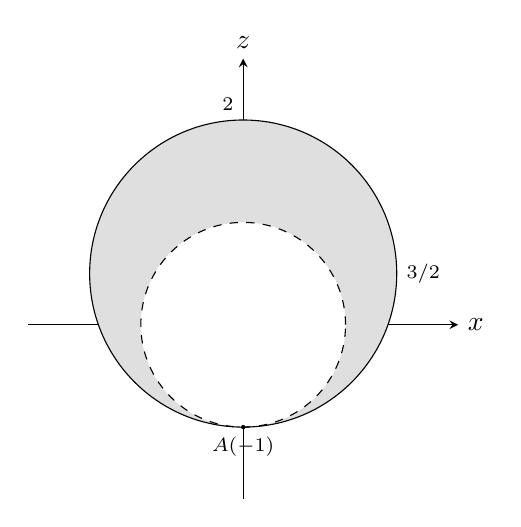
\begin{tikzpicture}[scale=1.3, >=stealth]
    \draw[->] (-2.1,0) -- (2.1,0) node[right] {$x$};
    \draw[->] (0,-1.7) -- (0,2.6) node[above] {$z$};
    \begin{scope}
      \clip (0,0.5) circle (1.5);
      \fill[gray!25] (0,0.5) circle (1.5);
      \fill[white] (0,0) circle (1);
    \end{scope}
    \draw (0,0.5) circle (1.5);
    \draw[dashed] (0,0) circle (1);
    \fill (0,-1) circle (0.6pt);
    \node[below] at (0,-1) {\scriptsize$A(-1)$};
    \node[right] at (1.5,0.5) {\scriptsize$3/2$};
    \node[above left] at (0,2) {\scriptsize$2$};
  \end{tikzpicture}
  \caption{$V$の$xz$平面での切断面（外側の円が半径$3/2$，中心$(0,1/2)$；内側の点線円が単位球$S$の断面，点$A$で内接）}
\end{figure}

この体積$V$は，$S$が半径$3/2$の球（中心$(0,0,1/2)$）に点$A$で内接し完全に含まれることから，
\begin{align*}
  V=\frac43\pi\left\{\left(\frac32\right)^3-1\right\}=\frac{19}6\pi<\frac{19}6\times3.15=\frac{19.95}2<10
\end{align*}
となる．

\bigskip

\subsection*{第4問}

\noindent
{\bf [解]}
$f(x)=\dfrac{x^2}{x^2+1}$，$f'(x)=\dfrac{2x}{(x^2+1)^2}$だから，$x=t$（$t\ne0$）での$C$の接線$\ell$の方向ベクトル$\vec\ell$は
\begin{align*}
  \vec\ell=
  \begin{pmatrix}1\\\dfrac{2t}{(t^2+1)^2}
  \end{pmatrix}
\end{align*}
である．また，
\begin{align*}
  \overrightarrow{PQ}=
  \begin{pmatrix}t\\\dfrac{t^2}{t^2+1}-a
  \end{pmatrix}
\end{align*}
だから，$PQ\perp\ell$となる時，
\begin{align*}
  \vec\ell\cdot\overrightarrow{PQ}=t+\frac{2t}{(t^2+1)^2}\left(\frac{t^2}{t^2+1}-a\right)=0\quad\cdots①
\end{align*}

①をみたす$t\ne0$の存在条件をもとめる．$t\ne0$だから，①を変形して，
\begin{align*}
  a=\frac12(t^2+1)^2+\frac{t^2}{t^2+1}
\end{align*}

$y=a$と$y=(\text{右辺})$が$t\ne0$に共有点をもてばよい．$p=t^2+1$とおくと，$t\ne0\iff p>1$であり，右辺を$g(p)$とおくと，
\begin{align*}
  g(p)=\frac12p^2+\frac{p-1}p=\frac12p^2+1-\frac1p
\end{align*}
\begin{align*}
  g'(p)=p+\frac1{p^2}
\end{align*}

$p>0$で$g'(p)>0$だから，$g(p)$は単調増加．したがって，もとめる条件は，$p>1$の範囲で$g(p)$が$a$の値をとることと同値で，$g$が$(1,\infty)$上連続かつ単調増加であることから，
\begin{align*}
  a>g(1)=\frac12
\end{align*}

\bigskip

\subsection*{第5問}

\noindent
{\bf [解]}
$Q_k(0,0,q_k)$とおく．$\triangle OP_kQ_k$に三平方の定理を用いて，
\begin{align*}
  1=q_k^2+\left(\frac kn\right)^2+\left(1-\frac kn\right)^2\quad\therefore\ q_k=\sqrt{2\cdot\frac kn-2\left(\frac kn\right)^2}\quad(>0)
\end{align*}

さらに，$\triangle OP_kP_{k+1}$の面積$S_k$は，サラスの公式により
\begin{align*}
  S_k=\frac12\left|\frac kn\left(1-\frac{k+1}n\right)-\frac{k+1}n\left(1-\frac kn\right)\right|=\frac12\cdot\frac1n
\end{align*}

だから，
\begin{align*}
  V_k=\frac13S_kq_k=\frac{\sqrt2}6\cdot\frac1n\sqrt{\frac kn-\left(\frac kn\right)^2}
\end{align*}

より，
\begin{align*}
  \lim_{n\to\infty}\sum_{k=0}^{n-1}V_k&=\frac{\sqrt2}6\int_0^1\sqrt{x-x^2}\,dx\\
  &=\frac{\sqrt2}6\int_0^1\sqrt{\frac14-\left(x-\frac12\right)^2}\,dx\\
  &=\frac{\sqrt2}{48}\pi
\end{align*}

\bigskip

\subsection*{第6問}

\noindent
{\bf [解]}
(1)
\begin{align*}
  1\text{回シャッフル}&\ \cdots\ \{5,1,6,2,7,3,8,4\}\\
  2\text{回シャッフル}&\ \cdots\ \{7,5,3,1,8,6,4,2\}\\
  3\text{回シャッフル}&\ \cdots\ \{8,7,6,5,4,3,2,1\}
\end{align*}
から，$\{8,7,6,5,4,3,2,1\}$．

(2) $\{1,2,\ldots,2N\}$を$t$回シャッフルした後における数$k$（$1\le k\le2N$）の位置を$f_t(k)$と表す．以下の漸化式を得る．
\begin{align*}
  1\le f_t(k)\le N\text{の時，}&\ f_{t+1}(k)=2f_t(k)\\
  N+1\le f_t(k)\le2N\text{の時，}&\ f_{t+1}(k)=2f_t(k)-(2N+1)
\end{align*}
$\cdots①$

（シャッフルでは，現在の並びの前半（位置$1,\ldots,N$）の$i$番目の数は新しい並びの位置$2i$に，後半（位置$N+1,\ldots,2N$）の$i$番目の数は新しい並びの位置$2i-1$に移ることによる．）

題意から，$f_0(k)=k$，$f_1(k)=f(k)$であるから，①より，
\begin{align*}
  1\le k\le N\text{の時，}&\ f(k)-2k=(2k-2k)=0\\
  N+1\le k\le2N\text{の時，}&\ f(k)-2k=(2k-2k)-(2N+1)=-(2N+1)
\end{align*}
となり，いずれも$f(k)-2k$は$2N+1$で割り切れる．$\blacksquare$

(3) 以下合同式の法を$2N+1=2^n+1$とする．①から，$1\le f_t(k)\le N$，$N+1\le f_t(k)\le2N$いずれの場合も
\begin{align*}
  f_{t+1}(k)\equiv2f_t(k)\pmod{2N+1}
\end{align*}
（わざわざ(2)を使えば，$f(k)\to f_{t+1}(k)$，$k\to f_t(k)$として同じ式を得る．）だから，くり返し用いて$f_0(k)=k$より，
\begin{align*}
  f_t(k)\equiv2^t\cdot k\pmod{2N+1}
\end{align*}

だから，$t=2n$として
\begin{align*}
  f_{2n}(k)\equiv2^{2n}k=\left(2^n\right)^2k\equiv\left((2^n+1)-1\right)^2k\equiv(-1)^2k=k\pmod{2N+1}
\end{align*}

ここで，$1\le k\le2N$，$1\le f_{2n}(k)\le2N$だから，法が$2N+1$であること（区間の幅$2N$が法より小さいこと）より，合同から等号が従い，
\begin{align*}
  f_{2n}(k)=k
\end{align*}

したがって，題意は示された．$\blacksquare$

\end{document}
